\section{Motivation}
\label{sec:motivation}

To motivate the need for considering user objectives, workflow behaviors, and CPU load in dynamic compression decisions, we examine the effects of transparent, asynchronous compression at different points in a producer-consumer pipeline. We use a representative scientific workflow consisting of a Gray-Scott reaction-diffusion simulation (producer) that generates time-series data, and an analysis program (consumer) that computes probability density functions from the simulation output. Both programs run simultaneously in a streaming fashion, with compression operating asynchronously to overlap communication with computation. This scenario is representative of many scientific computing workflows where simulations produce data faster than it can be consumed, necessitating compression to reduce storage and network transfer costs.

Figure~\ref{fig:contention_results} presents the compression performance characteristics when compression is performed at the producer (with CPU contention from the ongoing simulation) versus at the consumer (with idle CPU resources). The results reveal two critical insights that challenge the conventional view of compression as a purely data-dependent operation. First, compression performance depends significantly on the current load of the system, with CPU contention causing substantial slowdowns even when the compression operation itself runs asynchronously. For BZIP2, an archival compression method optimized for high compression ratios, the compression time increases by 1.61× when executed at the producer compared to the consumer. This slowdown occurs because the asynchronous compression thread contends with the simulation's compute phase for shared resources including CPU cores, memory bandwidth, and cache capacity. Even with careful thread placement, the compute-intensive nature of both the simulation and compression creates unavoidable interference. The contention effects are even more severe for certain algorithms: Snappy shows a 3.99× slowdown despite being designed for speed, while compute-intensive compressors like LZMA (1.23×) and BROTLI (1.31×) also experience significant degradation. This load-dependent performance variation means that predicting compression time requires not only understanding the algorithm and data characteristics, but also the current system state and resource availability.

\begin{figure}[htbp]
\centering
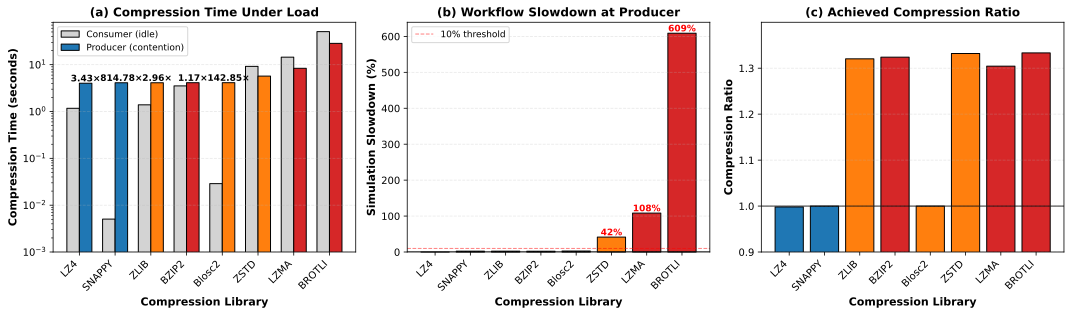
\includegraphics[width=0.95\textwidth]{motivation/contention_results.pdf}
\caption{Compression performance under different system loads in a Gray-Scott producer-consumer workflow. (a) Compression time for various algorithms when executed at the producer (with CPU contention) versus consumer (idle resources), showing up to 4× slowdown under contention. (b) Simulation slowdown caused by compression at the producer, with archival methods like BROTLI causing 456\% slowdown due to severe resource contention. (c) Compression ratios achieved by different algorithms, demonstrating the trade-off between compression quality and sensitivity to system load.}
\label{fig:contention_results}
\end{figure}

Second, workflow performance depends critically on both compression choice and compression location, creating complex optimization trade-offs that cannot be resolved by static policies. Archival compression methods such as LZMA (1.70× compression ratio) and Blosc2 (1.56×) achieve better compression compared to performance-driven compressors like LZ4 and Snappy (1.00×, essentially no compression), but require 10-1000× longer compression times. When archival compression is performed at the producer during periods of high CPU utilization, the combination of long compression time and contention-induced slowdown creates severe straggler effects: BROTLI causes 456\% simulation slowdown, effectively quintupling the workflow execution time, while LZMA and ZSTD cause 13.7\% and 11.7\% slowdowns respectively. The compression operation becomes a bottleneck that delays subsequent simulation steps, increasing overall workflow makespan despite the benefit of reduced data transfer time. However, when the same archival compression is performed at the consumer where CPU resources are underutilized, the increased compression time is hidden by the parallelism of the pipeline, and the superior compression ratio translates directly into reduced network transfer and storage costs without penalizing workflow completion time. Conversely, lightweight compressors that prioritize speed over compression ratio are ideal for producer-side compression under load, as their minimal CPU requirements and low sensitivity to contention allow them to reduce data transfer costs without creating pipeline bottlenecks. The optimal compression strategy therefore depends on a multi-dimensional assessment of the compression algorithm's characteristics (time, ratio, CPU intensity), the current system state (available CPU resources, memory bandwidth, cache pressure), and the workflow structure (pipeline parallelism, data transfer bottlenecks, end-to-end latency requirements). Static compression policies that ignore system load or workflow context will inevitably select suboptimal strategies, either choosing slow archival methods during resource contention (causing straggler effects) or choosing fast lightweight methods during resource abundance (missing opportunities for better compression). This motivates the development of adaptive compression systems that dynamically select algorithms and compression locations based on real-time system state and workflow requirements, using predictive models to balance compression ratio, time, quality, and resource utilization trade-offs in a context-aware manner.
